\documentclass[12 pt,a4paper]{article}
\usepackage[left=1.5cm,right=1.5cm,top=1.5cm,bottom=2cm]{geometry}
\input{stage1.sty}%
% Fichier de style stage2.sty [UTF8]
% Copyleft Laurent Bretonnière, laurent.bretonniere@gmail.com
% Version du 16/03/2015

\usepackage{mathtools}%	
\usepackage{fancybox}%
\usepackage{lastpage}%

\usepackage{fancyhdr}%
\renewcommand{\headrulewidth}{0.8pt}%
\renewcommand{\footrulewidth}{0.8pt}%

\usepackage[tikz]{bclogo}%
\renewcommand\bcStyleTitre[1]{\normalsize\textbf{#1}\smallskip}%
\renewcommand\logowidth{0pt}%

\newcommand{\fin}{\begin{center}%
$\clubsuit\clubsuit\clubsuit$%
\end{center}}%

\newcommand{\un}{\ding{192}\xspace}%
\newcommand{\deux}{\ding{193}\xspace}%
\newcommand{\trois}{\ding{194}\xspace}%
\newcommand{\quatre}{\ding{195}\xspace}%
\newcommand{\cinq}{\ding{196}\xspace}%
\newcommand{\six}{\ding{197}\xspace}%
\newcommand{\sept}{\ding{198}\xspace}%
\newcommand{\huit}{\ding{199}\xspace}%
\newcommand{\neuf}{\ding{200}\xspace}%

\setlength{\headheight}{15pt}%

%*********************************************************************************************
% Cours
%*********************************************************************************************

\usepackage[Lenny]{fncychap}%
\ChNumVar{\fontsize{76}{80}\usefont{OT1}{pzc}{m}{n}\selectfont}%
\ChTitleVar{\raggedleft\Huge\sffamily\bfseries}%

\renewcommand{\thesection}{\Roman{section})}%
\renewcommand{\thesubsection}{\arabic{subsection})}%
\renewcommand{\thesubsubsection}{\alph{subsubsection})}%

%*********************************************************************************************
% Environnements prédéfinis BCLOGO
%*********************************************************************************************

%% Lemme
\newenvironment{lem}{\begin{bclogo}[couleurBord=black!50,arrondi=0.1,logo=\hspace{17pt},barre=none]{Lemme :}}{\end{bclogo}\medskip}%

%% Propriété
\newenvironment{prop}[1][]{\begin{bclogo}[couleur=black!10,couleurBord=black!50,arrondi=0.1,logo=\hspace{17pt},barre=none]{Propriété :~#1}}{\end{bclogo}}%

%% Théorème
\newlength{\textlarg}
\settowidth{\textlarg}{~}
\newenvironment{theo}[1][\hspace{-\textlarg} :]{\begin{bclogo}[couleur=black!5,couleurBord=black!50,arrondi=0.1,logo=\hspace{17pt}, barre=none]{Théorème~#1}}{\end{bclogo}\medskip}%

\newenvironment{theon}[1][]{\begin{bclogo}[couleur=black!5,couleurBord=black!50,arrondi=0.1,logo=\hspace{17pt}, barre=none]{Théorème :~#1}}{\end{bclogo}\medskip}%

%% Corollaire
\newenvironment{coro}[1][]{\begin{bclogo}[couleurBord=black!50,arrondi=0.1,logo=\hspace{17pt},barre=none]{Corollaire :~#1}}{\end{bclogo}\medskip}%

%% Définition(s)

\newenvironment{defi}{\begin{bclogo}[couleur=black!10,couleurBord=black!50,arrondi=0.1,logo=\hspace{17pt}, barre=none]{Définition :}}{\end{bclogo}\medskip}%

\newenvironment{defis}{\begin{bclogo}[couleurBord=black!50,arrondi=0.1,logo=\hspace{17pt}, barre=none]{Définitions :}}{\end{bclogo}\medskip}%

%% Preuve
\newenvironment{pf}{\renewcommand\logowidth{17pt}\begin{bclogo}[noborder=true,logo=\hspace{17pt},couleurBarre=black!25,epBarre=3.5]{Démonstration :}}{\hspace*{\fill}$\Box$\end{bclogo}\smallskip\renewcommand\logowidth{0pt}}%

%\blacksquare

%% Notation
\newenvironment{nota}{\begin{bclogo}[couleurBord=black!50,arrondi=0.1,logo=\hspace{17pt},barre=none]{Notation :}}{\medskip}%

%% Exercice et Exercice-type
\newenvironment{exo}{$\circledast$ \quad\textsc{\underline{exercice} :}~}{\hspace*{\fill}$\circledast$\vskip 8pt}
\newenvironment{type}{$\blacktriangleright$ \quad\textsc{exercice-type :}~}{\hspace*{\fill}$\blacktriangleleft$\vskip 8pt}

%% Exemple(s)
\newenvironment{exem}{\textbf{Exemple :}~}{\medskip}
\newenvironment{exems}{\textbf{Exemples :}~}{\medskip}

%% Remarque(s)
\newenvironment{rem}{\textbf{Remarque :}~}{\medskip}
\newenvironment{rems}{\textbf{Remarques :}~}{\medskip}

%% Rappel(s)
\newenvironment{rap}{\textbf{Rappel :}~}{\medskip}
\newenvironment{raps}{\textbf{Rappels :}~}{\medskip}

%% Cas particulier(s)
\newenvironment{cp}{\textbf{Cas particulier :}~}{\medskip}
\newenvironment{cps}{\textbf{Cas particuliers :}~}{\medskip}

%% Application
\newenvironment{appli}{\textbf{Application :}~}{\medskip}%{\medskip} %
\usepackage{pgf,tikz}
\usetikzlibrary{arrows}
%\pagestyle{empty}
\usepackage{multicol}
\usepackage{setspace}
\renewcommand{\baselinestretch}{1.1}% interligne
\setlength{\columnseprule}{1pt} % trait de séparation entre les colonnes
\setlength{\columnsep}{10pt} % Espace entre les colonnes 
\usetikzlibrary{patterns}

\pagestyle{fancy}
\fancyhead{}
\renewcommand{\headrulewidth}{0pt}
%\lfoot{Chapitre 1}
\cfoot{\thepage}
%\rfoot{suites}


%\usepackage{hyperref}
\begin{document}

$2^{de}$\hfill {\LARGE Fonctions affines} \hfill déc 2020
\trait

\section{\underline{Définition et  propriétés}}
\begin{defi}
Une fonction $f$ est une fonction affine ssi $f$ est définie sur $\R$ par $f(x)=mx+p$\medskip\\ ($m$ et $p$ étant des nombres réels constants).\medskip\\
Le nombre $m$ est le coefficient directeur et $p$ est l'ordonnée à l'origine.\medskip\\
$\bullet$ si $m=0$ alors $f(x)=p$, alors $f$ est une fonction constante.\medskip\\
$\bullet$ si $p=0$ alors $f(x)=mx$, alors $f$ est une fonction linéaire.\medskip
\end{defi}

\underline{Exemples :} $f:x\longmapsto 2x+3$ est affine. $g:x \longmapsto -5x$ est linéaire. $h:x\longmapsto7$ est une fonction constante (toutes les trois sont affines).\medskip
\begin{prop}
La représentation graphique d'une fonction affine est une droite.\medskip\\ 
$\bullet$ si la fonction est constante, alors cette droite est parallèle à l'axe des abscisses.\medskip\\
$\bullet$ si la fonction est linéaire, alors cette droite passe par l'origine du repère\medskip\\
(car $f(0)=m\x0=0$ donc la droite passe par le point de coordonnées (0;0)).
\end{prop}

\underline{Exemples :} Construire la représentation graphique de $f$, $g$, $h$ et $k$ définies par $f(x)=\frac{4}{5}x-3$, $g(x)=2x$, $h(x)=-\frac{4}{3}x+1$ et $k(x)=-3$.\medskip\\
La dernière est horizontale au niveau de l'ordonnée $-3$. Pour les autres on peut construire un tableau de valeurs (au moins 2 abscisses choisies pour calculer l'image).

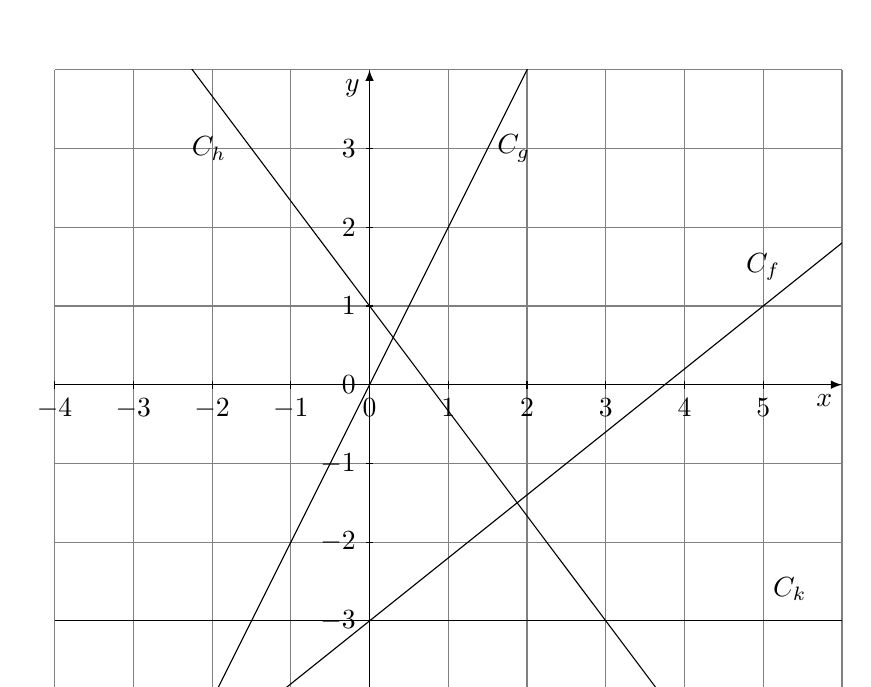
\begin{tikzpicture}[x=10mm,y=10mm]
\draw [gray,xstep=1,ystep=1] (-4,-4) grid (6,4);
\draw [->,>=latex] (-4,0) -- (6,0) node [below left] {$x$};
\draw [->,>=latex] (0,-4) -- (0,4) node [below left] {$y$};

\foreach \x in {-4,...,5}
\draw (\x,0.5mm) -- (\x,-0.5mm) node [below] {$\x$};
\foreach \y in {-3,...,3}
\draw (0.5mm,\y) -- (-0.5mm,\y) node [left] {$\y$};

%\draw (0,0) node [below left] {$O$};

\clip (-4,-4) rectangle (6,4);
\draw [domain=-4:10,samples=100] plot (\x, 0.8*\x-3);
\draw (1.5,3) node [right] {$\mathscr{C}_g$};
\draw [domain=-4:10,samples=100] plot (\x, 2*\x);
\draw [domain=-4:10,samples=100] plot (\x, -1.333*\x+1);
\draw [domain=-4:10,samples=100] plot (\x, -3);
\draw (5,1.2) node [above] {$\mathscr{C}_f$};
\draw (-1.7,3) node [left] {$\mathscr{C}_h$};
\draw (5,-2.6) node [right] {$\mathscr{C}_k$};
\end{tikzpicture}

\newpage

\underline{Exercice :} Déterminer les coordonnées du points d'intersection entre les droites $\mathscr{C}_f$ et $\mathscr{C}_g$:\medskip\\
Pour trouver l'abscisse du point d'intersection, on résout : \medskip\\
$f(x)=g(x)=\iff \frac{4}{5}x-3=2x\iff \frac{4}{5}x-2x=3\iff \frac{4}{5}x-\frac{10}{5}x=3\iff \frac{-6}{5}x=3$\medskip\\
$\iff x=3\x\frac{-5}{6}=-\frac{5}{2}$\medskip\\
ordonnée : $g(-\frac{5}{2})=2\x\frac{-5}{2}=-5$\medskip\\
Le point d'intersection a pour coordonnées $(-\frac{5}{2};-5)$.

\begin{prop} Soit $f$ une fonction affine ($f(x)=mx+p$)\\
Soient $x_1$ et $x_2$ deux nombres réels distincts, alors le rapport $\frac{f(x_2)-f(x_1)}{x_2-x_1}$ est constant et est égal au coefficient directeur $m$.\medskip
\end{prop}

\begin{pf}
$\frac{f(x_2)-f(x_1)}{x_2-x_1}=\frac{mx_2+p-(mx_1+p)}{x_2-x_1}=\frac{mx_2+p-mx_1-p}{x_2-x_1}=\frac{mx_2-mx_1}{x_2-x_1}$\medskip\\
$=\frac{m(x_2-x_1)}{(x_2-x_1)}=m$\hspace{3cm} (en simplifiant par $(x_2-x_1)$)
\end{pf}

\underline{Remarque1 :} la propriété précédente peut servir à calculer le coefficient directeur avec deux points\medskip\\
de la droite. Exemple : déterminer la fonction affine $f$ telle que $f(-2)=4$ et $f(5)=2$\medskip\\
coefficient directeur:$m=\frac{f(x_2)-f(x_1)}{x_2-x_1}=\frac{2-4}{5-(-2))}=\frac{-2}{7}$\medskip\\
donc $f(x)=-\frac{2}{7}x+p$ (avec $p\in\R$)\medskip\\
or $f(-2)=4$ donc $-\frac{2}{7}\x (-2)+p=4$ donc $\frac{4}{7}+p=4$ donc $p=4-\frac{4}{7}=\frac{28}{7}-\frac{4}{7}=\frac{24}{7}$\\D'où $f(x)=-\frac{2}{7}x+\frac{24}{7}$

\underline{Remarque2 :} si on connait 2 points $A(x_A;y_A)$  et $B(x_B;y_B)$ de la droite $\mathscr{C}_f$ alors $\boxed{m=\frac{y_B-y_A}{x_B-x_A}}$\medskip\\
(à connaître PAR COEUR)\medskip\\
Exemple : déterminer la fonction affine $f$ dont la courbe passe par $A(3;1)$ et $B(-3;-4)$\medskip\\
coefficient directeur:$m=\frac{y_B-y_A}{x_B-x_A}=\frac{-4-1}{-3-3}=\frac{-5}{-6}=\frac{5}{6}$\medskip\\
donc $f(x)=\frac{5}{6}x+p$ (avec $p\in\R$)\medskip\\
or $A(3;1)\in \mathscr{C}_f$ (traduction:$f(3)=1$) donc $\frac{5}{6}\x3+p=1$ donc $\frac{15}{6}+p=1$\medskip\\
donc $p=1-\frac{15}{6}=\frac{6}{6}-\frac{15}{6}=-\frac{9}{6}=-\frac{3}{2}$. D'où $f(x)=\frac{5}{6}x-\frac{3}{2}$\medskip\\
\underline{Remarque3 :} le coefficient directeur est  $\boxed{m=\frac{f(x_2)-f(x_1)}{x_2-x_1}=\frac{\textbf{écart des ordonnées}}{\textbf{écart des abscisses}}}$.\medskip\\
Donc, si on choisit un écart d'abscisses égal à 1, alors l'écart des ordonnées est égal directement à $m$.\medskip\\
Concrètement, si par exemple $m=3=\frac{3}{1}$, à partir d'un point connu de la droite représentant $f$, on se décale d'une unité vers la droite, puis on "monte" de 3 unités pour obtenir un nouveau point.\medskip\\
Si $m=-\frac{2}{3}$ alors, à partir d'un point connu, on se décale de 3 unités vers la droite, puis on "descend"\medskip\\
de 2 unités pour obtenir un autre point de cette droite.

\bigskip
\section{\underline{Variation et signe d'une fonction affine}}
\begin{prop} Soit $f$ une fonction affine ($f(x)=mx+p$, $m$ étant le coefficient directeur)\medskip\\
$\bullet$ si $m>0$ alors $f$ est strictement croissante (la droite "monte").\medskip\\
$\bullet$ si $m<0$ alors $f$ est strictement décroissante (la droite "descend").\medskip
\end{prop}
\begin{pf} On étudie le cas où $m>0$ : \medskip\\
Soient deux abscisses distinctes $x_1$ et $x_2$ telles que $x_1<x_2$.\medskip\\
$m=\frac{f(x_2)-f(x_1)}{x_2-x_1}$. Or le dénominateur $x_2-x_1$ est strictement positif car $x_1<x_2$.\medskip\\
De plus, $m$ est strictement positif aussi (cas étudié), donc le numérateur $f(x_2)-f(x_1)$ est forcément aussi strictement positif, ce qui veut dire que $f(x_1)<f(x_2)$, donc $f$ est strictement croissante (démonstration analogue si $m<0$).
\end{pf}

\underline{Tableau de signe d'une expression affine :} $-2x+8$ (exemple)\medskip\\
On cherche d'abord la valeur d'annulation, on résout donc:\medskip\\
$-2x+8=0\iff -2x=-8\iff x=\frac{-8}{-2}=4$
\[\begin{array}{|c|ccccc|}
\hline
x & -\infty & & 4 & & +\infty\\ \hline
\text{signe de } -2x+8 & & + & 0 & - & \\
\hline
\end{array}\]
Rq: c'est $+0-$ car la droite "descend" ($m=-2<0$), sinon c'est $-0+$ quand $m>0$. La ligne de signes représente le signe des ordonnées.\bigskip

\underline{Tableau de signe d'un produit de deux expressions affines :} $(-2x+8)(3x+5)$ (exemple)\medskip\\
On cherche d'abord les valeurs d'annulation, on résout donc 2 équations:\medskip\\
$ \bullet -2x+8=0\iff -2x=-8\iff x=\frac{-8}{-2}=4$\medskip\\
$ \bullet\hspace{0,2cm} 3x+5=0\iff 3x=-5\iff x=-\frac{5}{3}$\medskip

\begin{array}{|c|ccccccc|}
\hline
x & -\infty & & -\frac{5}{3} & & 4 & & +\infty\\ \hline
-2x+8 & & + & & + & 0 & - & \\
\hline
3x+5 & & - & & - & 0 & + & \\
\hline
(-2x+8)(3x+5) & & - & 0 & + & 0 & - & \\
\hline
\end{array}\medskip\\
\underline{Rq1:} ce tableau signifie que l'expression est strictement négative sur $]-\infty;-\frac{5}{3}[\cup]4;+\infty[$, strictement positive sur $]-\frac{5}{3};4[$ (et les valeurs d'annulation sont $-\frac{5}{3}$ et 4).\medskip\\
\underline{Rq2:} Un tableau de signe est utilisé pour résoudre une inéquation car "<0" signifie "strictement négatif" et ">0" signifie "strictement positif"\medskip\\
Dans l'exemple ci-dessus, on peut alors donner l'ensemble des solutions de, par exemple : \medskip\\
$(-2x+8)(3x+5)<0$ : $S=]-\infty;-\frac{5}{3}[\cup]4;+\infty[$\medskip\\
$(-2x+8)(3x+5)\geqslant0$ : $S=[-\frac{5}{3};4]$
\medskip
\underline{Rq3:} Parfois, il faut factoriser afin de se ramener à un produit pour pouvoir construire le tableau de signe.\medskip\\

\underline{Tableau de signe d'un quotient de deux expressions affines :} $\frac{-2x+8}{3x+5}$ (exemple)\medskip\\
la valeur d'annulation du numérateur est aussi celle de la fraction (ici 4) et la valeur d'annulation du dénominateur est une valeur interdite (sinon division par zéro)(ici $-\frac{5}{3}$).\medskip\\
Le seul changement par rapport au produit, c'est qu'il faut symboliser la valeur interdite par ||.

\[\begin{array}{|c|ccccccc|}
\hline
x & -\infty & & -\frac{5}{3} & & 4 & & +\infty\\ \hline
-2x+8 & & + & & + & 0 & - & \\
\hline
3x+5 & & - & & - & 0 & + & \\
\hline
\frac{-2x+8}{3x+5} & & - & || & + & 0 & - & \\
\hline
\end{array}\]
\medskip
\underline{Rq1: } Une valeur interdite ne fait jamais partie d'un ensemble de solution.\medskip\\
\underline{Rq2: } Parfois, il faut mettre au même dénominateur pour pouvoir construire le tableau de signe.\medskip\\
\underline{Exemple: } Résoudre $\frac{3x-2}{2x+7}\geqslant3$
Valeur interdite : $2x+7=0\iff x=-\frac{7}{2}$.\medskip\\
Pour $x\neq -\frac{7}{2}$, $\frac{3x-2}{2x+7}\geqslant3\iff \frac{3x-2}{2x+7}-3\geqslant 0\iff \frac{3x-2-3(2x+7)}{2x+7}\geqslant 0$\medskip\\
$\iff \frac{3x-2-6x-21}{2x+7}\geqslant 0\iff \frac{-3x-23}{2x+7}\geqslant 0$\medskip\\
Valeur d'annulation : $-\frac{23}{3}$\medskip\\
\[\begin{array}{|c|ccccccc|}
\hline
x & -\infty & & -\frac{23}{3} & & -\frac{7}{2} & & +\infty\\ \hline
-3x-23 & & + & 0 & - & & - & \\
\hline
2x+7 & & - & & - & 0 & + & \\
\hline
\frac{-3x-23}{2x+7} & & - & 0 & + & || & - & \\
\hline
\end{array}\]
\medskip
L'ensemble des solutions est donc $S=[-\frac{23}{3};-\frac{7}{2}[$
\end{document}
